%! TeX root = master.tex
% !TEX program = lualatex

\lecture{5}{2026-10-08}{Introduction to applied cryptography}{}
\chapter{Applied Cryptography}
\label{ch:crypto}

\section{Introduction}

\subsection{Why does cryptography matter?}

Cryptography protects data in two situations:
\begin{itemize}
    \item \textbf{Data in transit}: securing communication (e.g.\ HTTPS, VPNs).
    \item \textbf{Data at rest}: securing stored information (e.g.\ encrypted backups, encrypted disks).
\end{itemize}

\begin{center}
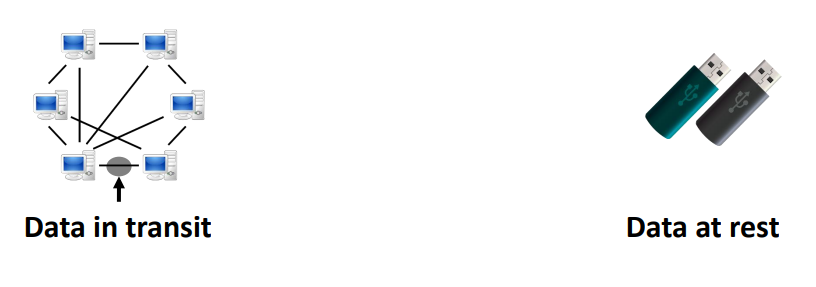
\includegraphics[width=0.6\linewidth]{images/img_20261031_181014.png}
\end{center}

Cryptography is historically born from the quest for \textbf{confidentiality} (information cannot be accessed by unauthorized parties), but it is also the building block for many other properties:
\begin{itemize}
    \item \textbf{Integrity}: ensuring data has not been tampered with (hashing, MACs, signatures);
    \item \textbf{Authentication}: verifying identity (protocols);
    \item but also \textbf{anonymity}, non-repudiation, etc.
\end{itemize}
This first lecture focuses on the basics of using cryptography for \textbf{confidentiality}. Integrity and authentication come in the following lectures.

\subsection{The core problem: secure communication over an insecure channel}

\begin{center}
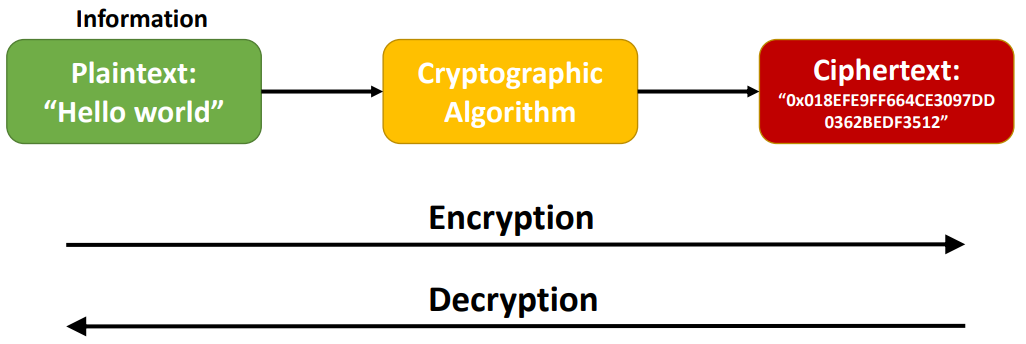
\includegraphics[width=0.7\linewidth]{images/img_20261031_181346.png}
\end{center}

We need a way for \textbf{Alice} to send a message to \textbf{Bob} such that \textbf{Eve} (the adversary, the \emph{eavesdropper}) \textbf{cannot read it}, even though Eve sees everything that goes over the channel.

\begin{remark}
Confidentiality of \textbf{data at rest} is a particular case where \textbf{Alice $=$ Bob}: Alice ``sends'' a message to her future self (the disk, the backup), and Eve is whoever gets access to the storage.
\end{remark}

\subsection{Encryption and decryption}

\begin{definition}[Encryption / decryption algorithm]
\begin{itemize}
    \item The \textbf{encryption algorithm} is a set of cryptographic instructions that converts a \textbf{plaintext} message into a \textbf{ciphertext}.
    \item The \textbf{decryption algorithm} is a set of cryptographic instructions that converts a \textbf{ciphertext} back into the \textbf{plaintext}.
\end{itemize}
Both algorithms require a \textbf{key}: encryption \textbf{cannot be reversed without the key}.
\end{definition}

Notation (cryptography as functions):
\begin{itemize}
    \item \textbf{Plaintext} $M$: the original message (e.g.\ ``Hello world'');
    \item \textbf{Key} $K$: a secret value;
    \item \textbf{Ciphertext} $C$: the scrambled message (e.g.\ \texttt{0x018EFE9FF664CE3097DD\dots}).
\end{itemize}
\[
\boxed{C = E_K(M) \qquad \text{and} \qquad M = D_K(C)}
\]
We also write $\mathrm{Enc}(k, m)$ and $\mathrm{Dec}(k, c)$.

\begin{center}
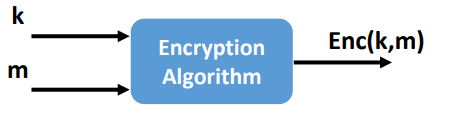
\includegraphics[width=0.45\linewidth]{images/img_20261031_181508.png}
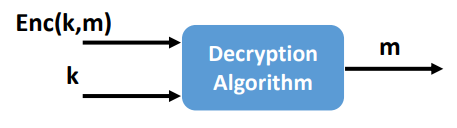
\includegraphics[width=0.45\linewidth]{images/img_20261031_181521.png}
\end{center}

\paragraph{Protocol for confidentiality.}
\begin{enumerate}
    \item Get a key $k$ \textbf{shared} between Alice and Bob.
    \item Alice encrypts the message: $m \mapsto \mathrm{Enc}(k, m)$.
    \item Alice sends $\mathrm{Enc}(k, m)$ over the insecure channel.
    \item Bob decrypts: $\mathrm{Dec}(k, \mathrm{Enc}(k,m)) = m$.
\end{enumerate}
Step 1 is far from trivial: it is the \textbf{key distribution problem}, solved in Section~\ref{sec:public-key} with public-key cryptography.

\subsection{The core requirements}

\begin{definition}[Correctness: invertibility]
The decryption function $D_K$ must be the inverse of $E_K$:
\[
\forall K, \forall M, \quad D_K(E_K(M)) = M.
\]
Otherwise, Bob cannot recover the original message $M$.
\end{definition}

\begin{definition}[Security requirement]
To provide security, $E_K$ must also be \textbf{hard to invert without knowing the key $K$}.
\end{definition}

\paragraph{Hard to invert: the key space.} Concretely, in an \textbf{ideal} cryptosystem, the only viable attack for Eve to find the plaintext $M$ must be to \textbf{try every single possible key $K$}: a \textbf{brute-force attack}. The goal of a secure scheme is to \textbf{force the attacker into this situation}. The \textbf{key space} (the set of all possible keys) must then be large enough to make brute force infeasible.

\begin{remark}[Eve knows the algorithm]
In all the examples below, Eve knows \emph{which} cipher is used (Caesar, substitution, OTP, \dots); only the \textbf{key} is secret. This is the \textbf{open design} principle seen in the security principles lecture (also known in cryptography as \emph{Kerckhoffs' principle}): the security must rest on the secrecy of the key, never on the secrecy of the design.
\end{remark}

\subsection{Bits of security}

\begin{definition}[Bits of security]
A scheme provides $N$ \textbf{bits of security} if the best known attack requires about $2^N$ operations (attempts). For an ideal scheme where brute force is the best attack, the bits of security equal $\log_2 |\mathcal{K}|$, where $|\mathcal{K}|$ is the size of the key space.
\end{definition}

\begin{itemize}
    \item \textbf{Goal}: an $N$-bit key should offer security \textbf{as close to $N$ bits as possible}, i.e.\ require $2^N$ attempts.
    \item \textbf{The break}: if a $1024$-bit key can be broken with only $2^{40}$ attempts ($40$ bits of security), the algorithm is \textbf{considered broken}, even if $2^{40}$ were still a lot of work.
\end{itemize}

\begin{remark}
\textbf{Key space size $\neq$ security.} A huge key space is \emph{necessary} (otherwise brute force works) but \emph{not sufficient}: a structural weakness can let the attacker skip almost all the keys. The two classical ciphers below illustrate exactly this.
\end{remark}

\section{Bad cryptography: classical ciphers}

These are examples of \textbf{bad} cryptography. They are pedagogically interesting because they introduce the first attack: \textbf{frequency analysis}.

\subsection{Caesar's cipher}

\begin{definition}[Caesar's cipher]
\begin{itemize}
    \item \textbf{Encryption}: shift each letter by a fixed number $K$ in the alphabet: $E_K(x) = (x + K) \bmod 26$.
    \item \textbf{Decryption}: shift each letter by $-K$: $D_K(y) = (y - K) \bmod 26$.
    \item \textbf{Key space}: only $25$ possible (non-trivial) keys.
\end{itemize}
\end{definition}

\begin{example}
With $K = 3$:
\[
\texttt{ATTACK AT DAWN} \;\xrightarrow{K=3}\; \texttt{DWWDFN DW GDZQ}
\]
(A$\to$D, T$\to$W, C$\to$F, K$\to$N, W$\to$Z, N$\to$Q.)
\end{example}

\paragraph{Security insight.} $\log_2 25 \approx \mathbf{4.6}$ \textbf{bits of security}: far too small for real-world use. Brute force (trying the 25 keys and reading which output is English) is already trivial. But there is an even better attack.

\subsubsection{Cryptanalysis: frequency analysis}

\begin{itemize}
    \item Eve knows that Alice wrote a \textbf{long-enough message} for Bob \textbf{in English}.
    \item She knows that the most frequent letter in English is `\texttt{e}'.
    \item She identifies the \textbf{most frequent letter in the ciphertext}: it likely corresponds to `\texttt{e}'.
    \item She directly recovers the key: $K = (\text{most frequent ciphertext letter}) - \texttt{e} \pmod{26}$.
\end{itemize}

This is a \textbf{frequency analysis attack}: the $25$ keys are reduced to \textbf{one} likely candidate, without any brute force.

\subsection{The substitution cipher}

Maybe the problem was having only $25$ keys? Let us use many more.

\begin{definition}[Substitution cipher]
Each letter is mapped to a unique, different letter, defined by a \textbf{permutation of the 26 letters}. The key is the permutation. Decryption applies the inverse permutation.
\end{definition}

\begin{example}
\begin{center}
\begin{tabular}{@{}ll@{}}
Plain alphabet: & \texttt{ABCDEFGHIJKLMNOPQRSTUVWXYZ} \\
Key (permuted): & \texttt{HOWBUGIACRYEVZXPJQMSNTFDKL}
\end{tabular}
\end{center}
\[
\texttt{hello world} \;\longrightarrow\; \texttt{aueex fxqeb}
\]
(h$\to$a, e$\to$u, l$\to$e, o$\to$x, w$\to$f, r$\to$q, d$\to$b.)
\end{example}

\paragraph{From 25 keys to $\approx 4 \times 10^{26}$ keys.}
\begin{itemize}
    \item Number of keys: $26! \approx 4.03 \times 10^{26}$ ($\approx 403$ septillion).
    \item Bit security: $\log_2 26! \approx \mathbf{88.4}$ \textbf{bits}?
    \item This key space \emph{looks} big enough (brute force is infeasible), but the cipher is \textbf{still easily broken by the same frequency analysis}.
\end{itemize}

\subsubsection{Cryptanalysis: the flaw, again}

\begin{itemize}
    \item \textbf{Vulnerability}: the cipher \textbf{preserves the statistical properties of the plaintext language} (single-letter frequencies, but also frequent pairs like ``th'', frequent words like ``the'', double letters, \dots).
    \item If Eve has a long enough ciphertext $C$, statistical analysis breaks the cipher, rendering the full $26!$ key space irrelevant.
\end{itemize}

\begin{remark}[The goal of the adversary may be smaller]
The adversary does not necessarily want the \textbf{full key}:
\begin{itemize}
    \item she might only recover \textbf{part of the key} (the mapping of a subset of letters), which may be enough to read most of the text;
    \item sometimes her goal is even smaller: she only wants to know whether Alice sent ``\texttt{Yes}'' or ``\texttt{No}'' to Bob. With Caesar or substitution, the \textbf{length} and \textbf{letter pattern} of the ciphertext already tell her.
\end{itemize}
A secure scheme must prevent \emph{any} information leak about the plaintext, not only the full recovery of the key.
\end{remark}

\begin{table}[h]
\centering
\begin{tabular}{@{}lccc@{}}
\toprule
\textbf{Cipher} & \textbf{Key space} & \textbf{Nominal security} & \textbf{Effective security} \\
\midrule
Caesar & $25$ & $\approx 4.6$ bits & $\approx 0$ bits (1 guess by frequency analysis) \\
Substitution & $26! \approx 4 \times 10^{26}$ & $\approx 88.4$ bits & a few tries (frequency analysis + dictionary) \\
\bottomrule
\end{tabular}
\caption{Bits of security versus key space size for the classical ciphers.}
\end{table}

\section{Adversaries in cryptography}

As always in computer security, the security of a scheme is \textbf{always measured relative to the power of the adversary} (the threat model). The general principle of the course still applies: security is studied against a \textbf{strategic adversary} that is given \textbf{limited, well-defined resources}. Here are the typical threat models in cryptography.

\subsection{Passive eavesdropping (ciphertext-only)}

In the Caesar and substitution examples, Eve's capabilities were very limited:
\begin{itemize}
    \item she \textbf{observed a long-enough ciphertext} $C$ corresponding to the encryption of a piece of English;
    \item and she had some compute power to test a few keys.
\end{itemize}
This is a \textbf{passive eavesdropper}: Eve can \textbf{only read the ciphertext} (in the literature, a \emph{ciphertext-only attack}). This is not the only possible adversary model.

\subsection{Active adversaries}

A \textbf{more active attacker} can somehow \textbf{influence the system}: convince Alice to send Bob very specific messages, look at Bob's screen for two minutes to see some decrypted messages, observe the precise time it takes Bob to run his algorithm, \dots: anything that goes beyond just observing the communication.

\subsubsection{Active Model 1: Known Plaintext Attack (KPA)}

\begin{definition}[Known Plaintext Attack]
Eve is given access to \textbf{multiple pairs $(M, C)$} of messages and their corresponding ciphertexts, all encrypted with the secret key $K$. From these pairs, she tries to find the key $K$ (or to decrypt \emph{other} messages encrypted under $K$). Eve does \textbf{not choose} which pairs she sees.
\end{definition}

\paragraph{Why is KPA realistic?} Encryption is very often applied to \textbf{structured data}:
\begin{itemize}
  \item \textbf{Standard headers}: many encrypted messages contain predictable headers (``\texttt{From:}'', a destination address in a packet, timestamps, file format headers, \dots);
  \item \textbf{Malicious Guessing}: if Eve guesses a message (or part of it) and observes its encryption, she obtains an $(M, C)$ pair.
\end{itemize}

\paragraph{KPA and the substitution cipher.} Under KPA, the substitution cipher becomes even more broken. If Eve knows that $M = \texttt{THE QUICK BROWN FOX}$, she \textbf{immediately recovers the mapping of many letters}, drastically reducing the effective key space, \textbf{without even doing a statistical analysis}. When Alice later reuses $K$, a significant part of the key has already leaked; with a dictionary, Eve recovers the rest in very few tries.

\subsubsection{Active Model 2: Chosen Plaintext Attack (CPA)}

\begin{definition}[Chosen Plaintext Attack]
Eve can somehow convince Alice (or the system) to encrypt \textbf{arbitrary messages chosen by Eve} with the secret key. More abstractly: for any chosen plaintext $m$, Eve gets $E_K(m)$. We say that Eve has access to an \textbf{encryption oracle}.
\end{definition}

\begin{remark}
In KPA, Eve does not get to choose which $(M, C)$ pairs she observes; in CPA she \emph{chooses} $m$ and gets $(m, E_K(m))$. CPA is therefore a \textbf{strictly stronger} adversary model than KPA (and KPA is stronger than ciphertext-only). A scheme secure under CPA is secure under KPA, not the converse.
\end{remark}

\paragraph{Why is CPA realistic?}
\begin{itemize}
    \item \textbf{Messaging app}: a secure messaging service (Signal, WhatsApp) encrypts messages with the sender's key. If Eve gets access to Alice's phone for a few minutes, she can send any data she chooses to Bob and observe the encryption: an $(M, C)$ pair of her choice.
    \item \textbf{Encryption API}: Eve may interact with an API endpoint where she provides data and receives the encrypted output.
\end{itemize}

\paragraph{CPA and the substitution cipher: complete break.} Eve chooses the plaintext
\[
M = \texttt{abcdefghijklmnopqrstuvwxyz}.
\]
The resulting ciphertext $C$ \textbf{is the entire key} (the full permutation), in \textbf{a single query}!

\subsubsection{Practical Threat Model Side-channel attacks}

\begin{definition}[Side-channel attack]
Eve is allowed not only to access an ideal oracle, but also to \textbf{measure physical characteristics of the actual implementation} while it is encrypting/decrypting:
\begin{itemize}
    \item \textbf{Timing attack}: Eve measures how long it takes for a given message to be encrypted or a ciphertext to be decrypted;
    \item \textbf{Power analysis}: Eve observes the energy consumed by the device (e.g.\ a credit card) while doing the crypto.
\end{itemize}
\end{definition}

\paragraph{Why are side channels realistic?}
\begin{itemize}
    \item \textbf{Malicious ownership}: you often \emph{own} a device (a phone, a smart card, an embedded chip) that holds keys belonging to \emph{another} principal (Google, your bank), which are meant to be unreadable to you. The adversary has physical access by design.
    \item \textbf{Example (DRM)}: the decryption key for Digital Rights Management content (a movie, a song) is embedded in your media player or console. By measuring power or timing, an attacker could extract that secret key.
\end{itemize}

\begin{remark}
Side channels attack the \emph{implementation}, not the mathematics: a cipher that is perfectly secure on paper can leak its key through timing or power consumption. Compare with the \textbf{timing covert channels} of the MAC lecture: the leak is in an observable side effect, not in the intended output.
\end{remark}

\section{Perfect secrecy and the One-Time Pad}

\subsection{Removing frequency analysis}

Frequency analysis works because the same plaintext letter is always encrypted to the same ciphertext letter. To remove it, we must make sure that \textbf{letters are not encrypted to the same values}. One way to do this: use a \textbf{random key as long as the message}, so that every part of the message is encrypted with a different piece of key. This long key is called a \textbf{one-time pad}.

\paragraph{Recall: XOR.} The bitwise exclusive or $\oplus$ satisfies:
\[
a \oplus 0 = a, \qquad a \oplus a = 0, \qquad a \oplus b = b \oplus a, \qquad (a \oplus b) \oplus c = a \oplus (b \oplus c),
\]
and therefore $\boxed{a \oplus b \oplus b = a}$.

\begin{definition}[One-Time Pad (OTP)]
\begin{itemize}
    \item \textbf{Key}: a string $k$ of \textbf{truly random} bits, \textbf{as long as the message}, \textbf{pre-shared} between Alice and Bob, and \textbf{used only once}.
    \item \textbf{Encryption}: translate the message into bits and XOR it with the key:
    \[
    \mathrm{Enc}(k, m) = m \oplus k.
    \]
    \item \textbf{Decryption}: XOR the ciphertext with the same key:
    \[
    \mathrm{Dec}(k, c) = c \oplus k = m \oplus k \oplus k = m.
    \]
\end{itemize}
\end{definition}

\begin{example}[Encrypting ``YEAH'']
YEAH in ASCII is \texttt{0x59454148}.
\begin{center}
\begin{tabular}{@{}lr@{}}
Message (YEAH) & \texttt{01011001 01000101 01000001 01001000} \\
OTP key $k$ & \texttt{01110101 00011101 01001010 01001010} \\
\midrule
$c = m \oplus k$ & \texttt{00101100 01011000 00001011 00000010} \\
\midrule
$c \oplus k$ & \texttt{01011001 01000101 01000001 01001000} = YEAH \\
\end{tabular}
\end{center}
Decryption gives back exactly the same bits as the message.
\end{example}

\subsection{Why is the OTP perfectly secure?}

Intuition: for any ciphertext $C$, \textbf{every possible plaintext $M$ (of the same length) is equally consistent}. Since the key is uniformly random, $C$ gives the adversary \textbf{zero new information} about $M$.

\begin{example}[Any plaintext fits any ciphertext]
The ciphertext $c = \texttt{00101100 01011000 00001011 00000010}$ above came from YEAH. But it could just as well be the encryption of NOPE (\texttt{0x4e4f5045}) under the key
\[
k' = \text{NOPE} \oplus c = \texttt{01100010 00010111 01011011 01000111}.
\]
Since all keys are equally likely, Eve has no way to tell whether Alice said ``YEAH'' or ``NOPE''. For every pair $(m, c)$ there is \textbf{exactly one} key $k = m \oplus c$ mapping $m$ to $c$.
\end{example}

\begin{definition}[Perfect secrecy]
An encryption scheme is \textbf{perfectly secret} if observing the ciphertext does not change the adversary's knowledge about the plaintext:
\[
\forall m, \forall c, \qquad P\big(M = m \mid E_K(M) = c\big) = P(M = m).
\]
\end{definition}

Here, the plaintexts $m$ follow some distribution $P(M = m)$ (e.g.\ ``Yes'' is more probable than ``Autobus''), and we assume that the key $K$ is \textbf{uniformly distributed} over $\{0,1\}^n$ and independent of $M$.

\paragraph{Proof that the OTP is perfectly secret.} Let $n$ be the message length. By the definition of conditional probability,
\[
P(M = m \mid E_K(M) = c) = \frac{P(M = m \,\cap\, E_K(M) = c)}{P(E_K(M) = c)}.
\]
\textbf{Numerator.} $E_K(m) = m \oplus K = c \iff K = m \oplus c$. So, using the independence of $M$ and $K$,
\[
P(M = m \,\cap\, M \oplus K = c) = P(M = m \,\cap\, K = m \oplus c) = P(M = m) \cdot P(K = m \oplus c).
\]
\textbf{Denominator.},
\[
P(E_K(M) = c) =  P(K = m \oplus c).
\]
Hence
\[
P(M = m \mid E_K(M) = c) = P(M = m). \qquad \square
\]

\begin{remark}
Perfect secrecy is an \textbf{information-theoretic} guarantee: it holds even against an adversary with \textbf{unlimited computing power}. Brute force is useless: trying all keys produces \emph{all} possible plaintexts, each equally plausible. This is the strongest possible form of confidentiality, and it costs a key as long as the message.
\end{remark}

\subsection{The key problem of the OTP}

\begin{center}
\fbox{\parbox{0.85\linewidth}{\centering The OTP requires keys that are \textbf{truly random}, \textbf{message-length}, and \textbf{used only once}.}}
\end{center}

\paragraph{The showstopper.} Securely pre-distributing message-length keys for real-world applications is \textbf{impractical}: to send 1\,GB of data, Alice and Bob must first exchange 1\,GB of secret key over a secure channel. One might then think: if it is hard to exchange keys, can I just reuse them? \textbf{No.}

\subsection{Key reuse: the ``two-time pad''}

One-time pads are called like this because they \textbf{must not be reused}. Suppose Alice encrypts two messages $M_1$, $M_2$ with the same key $K$:
\[
C_1 = M_1 \oplus K, \qquad C_2 = M_2 \oplus K.
\]
Eve XORs the two ciphertexts and \textbf{the key cancels out}:
\[
\boxed{C_1 \oplus C_2 = M_1 \oplus K \oplus M_2 \oplus K = M_1 \oplus M_2.}
\]
Eve cannot directly read $M_1$ or $M_2$, but she learns \textbf{their XOR}, which is information about the plaintexts. This information feeds frequency analysis and helps recover the messages themselves.

\begin{example}[Exercise from the lecture: key reuse on two 5-letter words]
Alice reuses $K$ to encrypt two single-word English messages of length 5, $M_1$ and $M_2$, producing $C_1 = M_1 \oplus K$ and $C_2 = M_2 \oplus K$. \textbf{Show that Eve can ``likely'' recover the key and the two messages.}

\textbf{Solution.}
\begin{enumerate}
    \item Eve computes $C_1 \oplus C_2 = M_1 \oplus M_2$ (the key cancels).
    \item She takes an \textbf{English dictionary of all 5-letter words} (a few thousand words $W$).
    \item For every pair $(W_1, W_2)$ of dictionary words, she checks whether $W_1 \oplus W_2 = C_1 \oplus C_2$. This is a few million cheap XORs.
    \item Since $M_1 \oplus M_2$ is 40 bits and real words are very constrained, \textbf{very few pairs} (likely only the right one, and its swap) match.
    \item She then recovers the key $K = C_1 \oplus M_1$, and can decrypt anything else encrypted with $K$.
\end{enumerate}
The word ``likely'' is because several pairs could in principle match; in practice the candidate set is tiny.
\end{example}

\subsection{The OTP does not provide integrity}

\begin{center}
\fbox{\parbox{0.85\linewidth}{\centering The OTP guarantees \textbf{confidentiality} (nobody can read it).\\ It does \textbf{NOT} guarantee \textbf{integrity} (nobody can tamper with it).}}
\end{center}

\paragraph{Bit-flipping attack.} Let $\Delta$ be any bit string (e.g.\ $\Delta = 100\dots0$ to flip the first bit).
\begin{enumerate}
    \item Eve intercepts $C$ and sends $C' = C \oplus \Delta$ to Bob.
    \item Bob decrypts:
    \[
    M' = C' \oplus K = M \oplus K \oplus \Delta \oplus K = M \oplus \Delta.
    \]
\end{enumerate}
\textbf{Result}: Eve successfully changed the message ($M'$ is $M$ with the bits of $\Delta$ flipped) \textbf{without knowing $K$}. We say the OTP is \textbf{malleable}.

\begin{remark}[Exam hints: confidentiality $\neq$ integrity]
\begin{itemize}
    \item Encryption alone \textbf{never} gives integrity. To detect tampering, one needs a separate mechanism (a \textbf{MAC} with a secret key, or a digital signature; next lectures). In a past MCQ, the correct way for Roberta to send $m$ with confidentiality \emph{and} integrity, with two pre-shared keys, was $\mathrm{Enc}(K_1, m), \mathrm{MAC}(K_2, \mathrm{Enc}(K_1, m))$: two \emph{different} keys, and the MAC computed over the ciphertext.
    \item \textbf{XOR with a known value hides nothing.} $x \oplus y$ protects $x$ only if $y$ is secret, uniformly random and used once. In the Final 2024, an IV computed as $k \oplus \mathrm{pad}(\text{time})$ instead of a hash was a vulnerability: the IV is not secret and the time is public, so anyone recovers $k = \mathrm{IV} \oplus \mathrm{pad}(\text{time})$.
\end{itemize}
\end{remark}

\section{From the OTP to stream ciphers}

\subsection{Symmetric cryptography}

In \textbf{symmetric} schemes, encryption of the plaintext and decryption of the ciphertext are done using \textbf{the same key}. Two main types:
\begin{itemize}
    \item \textbf{Block ciphers}: operate on fixed-size blocks (e.g.\ 128 bits). Example: \textbf{AES} (Advanced Encryption Standard).
    \item \textbf{Stream ciphers}: operate one bit/byte at a time, like a \textbf{pseudo-OTP}. Example: \textbf{ChaCha20}.
\end{itemize}
This lecture dives deeper into stream ciphers.

\begin{definition}[Symmetric cryptographic key]
A \textbf{fixed-size input} to symmetric cryptographic primitives. The \textbf{size of the key} influences the level of security provided. Its properties:
\begin{itemize}
    \item \textbf{Known to both parties}: the partners must agree on the key before starting to use the primitive.
    \item \textbf{Reused}: the key is pre-shared once and then reused (but keys do have a ``duration'': they are renewed after some time).
    \item \textbf{Secret}: revealing the key eliminates any protection provided by the primitive.
\end{itemize}
\end{definition}

\begin{remark}
Note the contrast with the OTP: a symmetric key is \textbf{short and reused}, whereas the OTP key is as long as the message and used once. The whole point of stream ciphers is to get (almost) OTP security from a short reusable key.
\end{remark}

\subsection{Stream ciphers: the pseudo-OTP}

A stream cipher attempts to \textbf{emulate the OTP's security while solving the key-length problem}.

\begin{definition}[Stream cipher]
\begin{enumerate}
    \item \textbf{Short key} $K$: Alice and Bob share a small, manageable key (much smaller than the message), which must be kept \textbf{secret}.
    \item \textbf{Keystream generator (KSG)}: takes $K$ and an \textbf{Initialization Vector (IV)} and produces an arbitrarily long, \textbf{pseudo-random} bit stream $S = \mathrm{stream}(K, \mathrm{IV})$.
    \item \textbf{Encryption}: $C = M \oplus S$, as with the OTP.
    \item \textbf{Decryption}: the receiver feeds the KSG with the shared key and the IV (the IV is \textbf{sent along with the ciphertext}, in the clear), recreates the same stream $S$, and computes $M = C \oplus S$.
\end{enumerate}
\end{definition}

\begin{center}
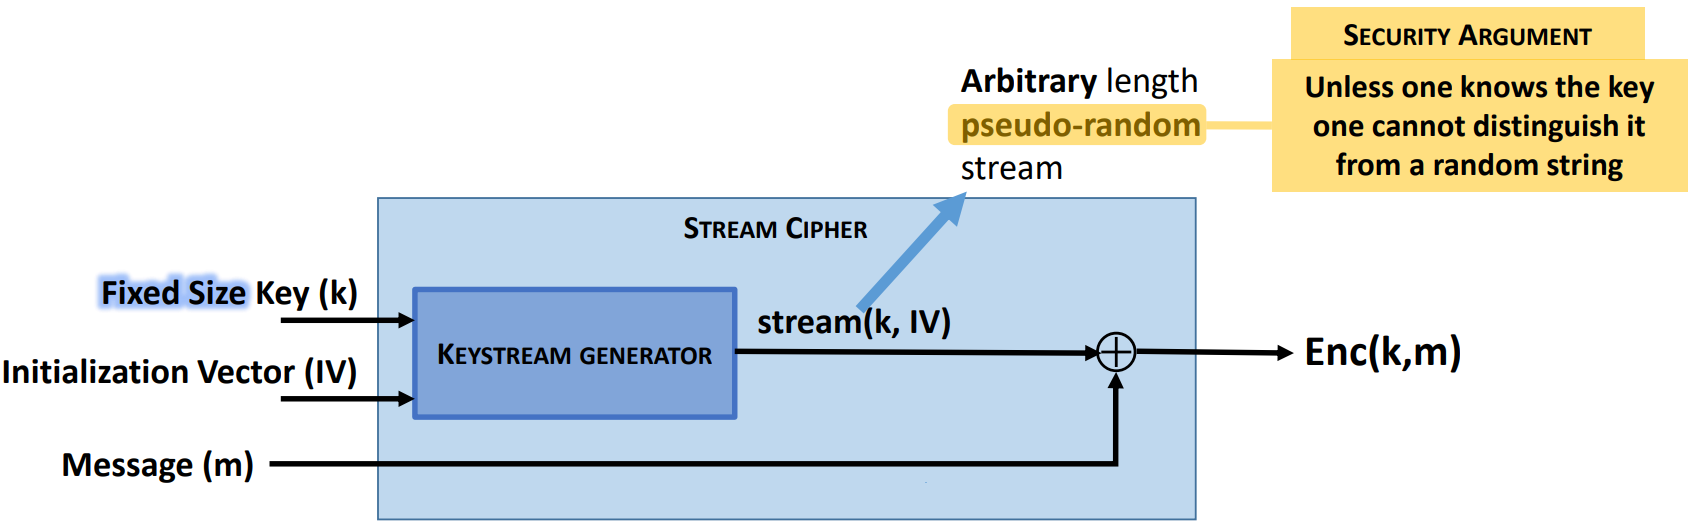
\includegraphics[width=\linewidth]{images/img_20261031_195042.png}
\end{center}

\paragraph{Security argument.} The output stream is \textbf{pseudo-random}: \textbf{unless one knows the key, one cannot distinguish it from a truly random string}. We generate potentially infinitely long ``randomness'' $S$ from a finite secret $K$, so the security depends entirely on $S$ being \textbf{computationally indistinguishable} from a truly random OTP key.

\begin{remark}[Perfect vs.\ computational security]
A stream cipher is \textbf{not} perfectly secret: the key is shorter than the message, so an unbounded adversary could try all $2^{|K|}$ keys and see which one gives a sensible plaintext. Its security is \textbf{computational}: breaking it should take about $2^{|K|}$ operations, which is infeasible for e.g.\ $|K| = 128$ or $256$.
\end{remark}

\subsubsection{Why does the KSG also take an IV?}

The key is \textbf{reused} across messages. Without an IV, the KSG would produce the \textbf{same stream $S$ for every message}, which is exactly a \textbf{reused one-time pad}: one could XOR two ciphertexts to get $C_1 \oplus C_2 = M_1 \oplus M_2$, recover the prefix of $S$ from any known plaintext ($S = C \oplus M$), and decode future messages. The IV makes sure that \textbf{two different messages are encrypted with two different streams}.

\begin{itemize}
    \item The IV does \textbf{not need to be secret} (it is sent in the clear with the ciphertext).
    \item It must \textbf{not be repeated} with the same key (otherwise the stream repeats and we are back to key reuse).
\end{itemize}

\subsubsection{Strengths and weaknesses}

\begin{table}[h]
\centering
\begin{tabular}{@{}p{4.2cm}p{9.2cm}@{}}
\toprule
\multicolumn{2}{@{}l}{\textbf{Weaknesses}} \\
\midrule
Low diffusion & A change in one plaintext bit only affects \textbf{one} ciphertext bit. \\
Susceptibility to modification & Low diffusion makes it easy to \textbf{tamper} with the message (bit flipping, exactly like the OTP). \\
\midrule
\multicolumn{2}{@{}l}{\textbf{Strengths}} \\
\midrule
Speed & Algorithms are \textbf{linear in time} and \textbf{constant in space}. \\
Low error propagation & An error in one bit (e.g.\ noise on the channel) does not affect the subsequent symbols. \\
\bottomrule
\end{tabular}
\caption{Stream ciphers: strengths and weaknesses.}
\end{table}

\subsubsection{Cryptanalysis: periodicity}

\begin{itemize}
    \item A keystream generator with a \textbf{finite state} (say $L$ bits) is \textbf{eventually periodic}: it has at most $2^L$ states, so after at most $2^L$ steps it revisits a state and from then on repeats.
    \item If the message is longer than the period, the stream repeats: two parts of the message are encrypted with the same stream, i.e.\ key reuse.
    \item \textbf{The attack}: if the period is identified and too small, knowing one period of the keystream (e.g.\ from a known plaintext) gives the keystream for the \textbf{entire message}.
\end{itemize}

\subsection{Interlude: building keystream generators}

\begin{remark}
You are \textbf{not expected to fully understand} this interlude: it illustrates design patterns for KSGs, the challenges of building secure ones, and the math needed to study them.
\end{remark}

\subsubsection{Linear Feedback Shift Registers (LFSR)}

\begin{definition}[LFSR]
A \textbf{linear recurrence relation}: the next output bit is a \textbf{linear function (XOR)} of previous bits. It extends an initial random sequence of bits (the state) into an arbitrarily long sequence of (maybe?) random-looking bits.
\end{definition}

\begin{example}
Initial state of 4 bits $a_0, \dots, a_3$ and recurrence $a_n = a_{n-3} \oplus a_{n-4}$. Starting from $1, 0, 0, 0$:
\[
a_4 = a_1 \oplus a_0 = 1,\quad a_5 = a_2 \oplus a_1 = 0,\quad a_6 = a_3 \oplus a_2 = 0,\quad a_7 = a_4 \oplus a_3 = 1,\quad a_8 = a_5 \oplus a_4 = 1, \dots
\]
Output sequence: $1, 0, 0, 0, 1, 0, 0, 1, 1, \dots$
\end{example}

\textbf{Advantage}: it uses only shift registers (state storage) and XOR gates (feedback), so it is \textbf{extremely fast and efficient in hardware}.

\paragraph{Randomness of LFSRs.}
\begin{itemize}
  \item \textbf{Maximal period}: if the characteristic polynomial (AICC1) of the recurrence is \textbf{primitive}, an $L$-bit register goes through the maximum possible number of states before repeating: $\mathbf{2^L - 1}$ (all states except the all-zero state, which is a fixed point: $0 \oplus 0 = 0$).
    \item \textbf{Distribution}: every non-zero state appears exactly once per cycle, so the output is highly \textbf{balanced}: over one cycle it contains exactly $2^{L-1}$ ones and $2^{L-1} - 1$ zeros.
\end{itemize}

\paragraph{Math danger.} Despite passing some statistical tests, an LFSR is \textbf{purely linear}. Algorithms like \textbf{Berlekamp--Massey} (beyond the scope of the class) recover the entire LFSR state, hence the whole keystream, from \textbf{a short segment of output} (about $2L$ bits, easily obtained with a known plaintext). \textbf{LFSRs must not be used directly as keystream generators}, though they have traditionally been used as \emph{building blocks} of KSGs.

\subsubsection{A5/1: a broken stream cipher}

\begin{itemize}
    \item Used historically to secure \textbf{GSM} mobile phone communications.
    \item Built by \textbf{combining multiple LFSRs in a non-linear way}, to overcome the linearity flaw while staying cheap and keeping the nice statistical properties.
    \item \textbf{The break}: despite the added complexity, mathematical weaknesses were found, allowing the cipher to be broken \textbf{much faster than brute force}.
\end{itemize}

\subsubsection{Non-broken stream ciphers}

There are modern stream ciphers for which there is \textbf{no known practical cryptanalysis}:
\begin{itemize}
    \item \textbf{Trivium}: based on three NLFSRs (non-linear variants of LFSRs) glued together with XOR and AND gates in a complex way;
    \item \textbf{Salsa20} (and its variant ChaCha20): using different techniques.
\end{itemize}

\subsection{Bit security and consequences: do not roll your own crypto}

\begin{itemize}
    \item \textbf{Cost of breaking}: exploiting a mathematical property or a bug can break a scheme \textbf{much faster than $2^{|K|}$} attempts, reducing its bit security.
    \item \textbf{The difficulty}: designing mathematically secure primitives, resistant to subtle attacks, is \textbf{incredibly hard}.
    \item \textbf{Conclusion}: \textbf{never design your own} stream cipher, block cipher, or hash function.
    \item \textbf{Best practice}: use \textbf{well-vetted, peer-reviewed, standard algorithms and their implementations} (AES, ChaCha20, SHA-3).
\end{itemize}

\begin{remark}
This is the same philosophy as for security models in the MAC lecture (``use a well-known model rather than inventing your own''), and an application of \textbf{open design}: standard algorithms are public and have survived years of public cryptanalysis, which is precisely what gives confidence in them.
\end{remark}

\section{Public-key cryptography}
\label{sec:public-key}

\subsection{Recap: the key distribution problem}

Symmetric ciphers are fast, but require a \textbf{pre-shared secret key}.

\textbf{Question}: how can Alice and Bob agree on a secret key if \textbf{all their communication is observed by Eve}?

\paragraph{The magic of asymmetric crypto.}
\begin{itemize}
    \item \textbf{The paradox}: before the 1970s, it was considered \textbf{impossible} to communicate securely without a pre-shared secret.
    \item \textbf{The revelation}: \textbf{public-key cryptography} allows two parties who have \textbf{never met} to establish a secure channel over a public one.
\end{itemize}

\subsection{Diffie--Hellman key exchange}

\begin{definition}[Diffie--Hellman (DH) key exchange]
\textbf{Public parameters}, known by Alice, Bob \emph{and Eve}: a large prime number $p$ and a generator $g$.

\begin{center}
\begin{tabular}{@{}p{6.5cm}p{6.5cm}@{}}
\toprule
\textbf{Alice} & \textbf{Bob} \\
\midrule
1. Chooses a private secret $a$. & 1. Chooses a private secret $b$. \\
2. Computes the public value $A = g^a \bmod p$. & 2. Computes the public value $B = g^b \bmod p$. \\
3. Sends $A$ to Bob. & 3. Sends $B$ to Alice. \\
4. Computes $K = B^a \bmod p$. & 4. Computes $K = A^b \bmod p$. \\
\bottomrule
\end{tabular}
\end{center}
\end{definition}

\paragraph{The shared secret.} Both obtain the same value:
\[
\boxed{K = B^a = (g^b)^a = g^{ba} = g^{ab} = (g^a)^b = A^b \pmod p}
\]
\begin{itemize}
    \item $K = B^a \bmod p$ is computable by \textbf{Alice} (she has the secret $a$ and received $B$);
    \item $K = A^b \bmod p$ is computable by \textbf{Bob} (he has the secret $b$ and received $A$);
    \item \textbf{Eve} sees $A$, $B$, $g$ and $p$, but \textbf{cannot compute $K$}: she has neither $a$ nor $b$, and cannot find them because of the \textbf{Discrete Logarithm Problem}.
\end{itemize}

\begin{definition}[Discrete Logarithm Problem]
Given $p$, $g$ and $A = g^a \bmod p$, find $a$. Computing $g^a \bmod p$ is easy (e.g.\ with \textbf{fast modular exponentiation}, square-and-multiply, in $O(\log a)$ multiplications), but there is \textbf{no known fast (polynomial) algorithm} to recover $a$ from $A$ and $p$ (nor $b$ from $B$).
\end{definition}

\begin{example}[Toy DH, with tiny numbers]
$p = 23$, $g = 5$. Alice picks $a = 6$, Bob picks $b = 15$.
\begin{itemize}
    \item $A = 5^6 \bmod 23 = 8$ \quad ($5^2 = 25 \equiv 2$, $5^4 \equiv 4$, $5^6 \equiv 4 \cdot 2 = 8$);
    \item $B = 5^{15} \bmod 23 = 19$;
    \item Alice: $K = B^a = 19^6 \bmod 23 = 2$; \quad Bob: $K = A^b = 8^{15} \bmod 23 = 2$.
\end{itemize}
Eve sees $p = 23$, $g = 5$, $A = 8$, $B = 19$. With such small numbers she can brute force $a$, but with $p$ of thousands of bits this is infeasible.
\end{example}

\subsection{Trapdoor (one-way) functions}

\begin{itemize}
    \item DH is one of many examples of how to use public-key cryptography to \textbf{establish a shared secret} (a shared key) that is then used for \textbf{symmetric cryptography}.
    \item Such schemes boil down to mathematical functions that are \textbf{easy to compute in one direction} but \textbf{hard (high complexity) to compute in the other direction}.
    \item For DH, the underlying difficulty is the \textbf{Discrete Logarithm Problem}.
\end{itemize}

\begin{remark}
Typical combination (\emph{hybrid encryption}): use slow public-key crypto only to agree on a short key, then encrypt the bulk of the data with fast symmetric crypto (AES, ChaCha20) under that key. This is how HTTPS, VPNs and messaging apps work.
\end{remark}

\subsection{Beyond Diffie--Hellman}

There are other ways to set up a shared secret (or even to directly communicate), all involving interesting mathematics:
\begin{itemize}
    \item \textbf{RSA}: based on the hardness of the \textbf{factoring} problem;
    \item \textbf{Elliptic Curve Cryptography (ECC)}: the discrete logarithm problem on elliptic curves instead of on integers modulo $p$ (smaller keys for the same security);
    \item \textbf{Post-Quantum Cryptography}: new primitives (e.g.\ \textbf{lattice} cryptography) designed to resist \textbf{quantum computers}, which could solve factoring and discrete log efficiently.
\end{itemize}

\subsection{Man-in-the-Middle (MITM) attack}

\paragraph{Vanilla DH is vulnerable to an active attack.} DH only guarantees \textbf{key agreement}, \textbf{not authenticity}: Alice does not verify \emph{who} she is agreeing with. DH is secure against a \emph{passive} eavesdropper, but not against an \emph{active} adversary who can intercept and replace messages.

\begin{enumerate}
    \item \textbf{Eve intercepts} $A$ from Alice and $B$ from Bob (they never reach their destination).
    \item \textbf{Eve impersonates} each party, using her own secret(s):
    \begin{itemize}
        \item Eve sends $E_B$ to Alice (pretending to be Bob). Alice computes a key $K_{AE}$, shared with Eve.
        \item Eve sends $E_A$ to Bob (pretending to be Alice). Bob computes a key $K_{BE}$, shared with Eve.
    \end{itemize}
    \item Eve now shares a key $K_{AE}$ with Alice and a separate key $K_{BE}$ with Bob. Each message from Alice is decrypted by Eve with $K_{AE}$, read (and possibly modified), re-encrypted with $K_{BE}$ and relayed to Bob, and vice versa.
\end{enumerate}

\textbf{Result}: Eve can \textbf{read, modify and relay all communication}, while Alice and Bob believe they have a private channel with each other.

\subsection{The need for trust (authentication)}

\begin{itemize}
    \item DH \textbf{solves the key distribution problem}, but creates the \textbf{identity verification problem}: is $B$ really Bob's?
    \item \textbf{Solution}: DH must be paired with a mechanism to \textbf{verify identity}, such as \textbf{digital signatures} (next lecture).
    \item \textbf{Setup}: parties still need to \textbf{trust a third party}, a \textbf{Certificate Authority} (CA), that vouches for the ownership of public keys.
\end{itemize}

\begin{remark}
This is exactly the ``integrity bootstraps confidentiality'' argument of the MAC lecture (PKI): perfect encryption is useless if the adversary can substitute her own key for Bob's. Confidentiality needs the \textbf{integrity / authenticity of the public values}.
\end{remark}

\section{Summary}

\begin{itemize}
    \item Cryptography protects data \textbf{in transit} and \textbf{at rest}; it builds confidentiality, integrity, authentication, anonymity. Core problem: Alice talks to Bob over a channel observed by Eve.
    \item Encryption: $C = E_K(M)$, $M = D_K(C)$. \textbf{Correctness}: $D_K(E_K(M)) = M$ for all $K, M$. \textbf{Security}: hard to invert without $K$; ideally, the only attack is \textbf{brute force} over the key space. Only the key is secret, not the algorithm (open design).
    \item \textbf{Bits of security}: the best attack costs $2^N$. A large key space is necessary but not sufficient: \textbf{Caesar} ($25$ keys, $4.6$ bits) and \textbf{substitution} ($26!$ keys, $\approx 88$ bits nominal) are both broken by \textbf{frequency analysis}, because they preserve the statistics of the language.
    \item \textbf{Adversary models}: passive eavesdropper (ciphertext only) $<$ \textbf{KPA} (known $(M, C)$ pairs, realistic due to structured data) $<$ \textbf{CPA} (encryption oracle; breaks substitution in one query). \textbf{Side channels} (timing, power) attack the implementation (DRM, smart cards).
    \item \textbf{One-Time Pad}: $c = m \oplus k$, $m = c \oplus k$, with $k$ truly random, as long as $m$, used once. \textbf{Perfect secrecy}: $P(M = m \mid C = c) = P(M = m)$, secure even against unbounded adversaries.
    \item OTP limits: \textbf{key distribution} of message-length keys is impractical; \textbf{key reuse} gives $C_1 \oplus C_2 = M_1 \oplus M_2$ (space trick, dictionary attack); \textbf{no integrity}: bit flipping $C \oplus \Delta \to M \oplus \Delta$ (malleability).
    \item \textbf{Symmetric crypto}: same key for encryption and decryption; short, reused, secret keys. Block ciphers (AES) vs.\ \textbf{stream ciphers} (ChaCha20).
    \item \textbf{Stream cipher}: $S = \mathrm{KSG}(K, \mathrm{IV})$, $C = M \oplus S$. Security is \textbf{computational}: $S$ indistinguishable from random without $K$. The \textbf{IV} (public, never repeated under the same key) avoids reusing the same stream. Low diffusion, malleable, fast, low error propagation. Finite state $\Rightarrow$ periodic.
    \item \textbf{LFSRs}: fast, period $2^L - 1$ and balanced if the polynomial is primitive, but \textbf{linear} (Berlekamp--Massey): only a building block. \textbf{A5/1} (GSM) broken; \textbf{Trivium}, \textbf{Salsa20/ChaCha20} not. \textbf{Never roll your own crypto}: use AES, ChaCha20, SHA-3.
    \item \textbf{Public-key crypto} solves key distribution. \textbf{Diffie--Hellman}: public $p, g$; $A = g^a$, $B = g^b$; $K = B^a = A^b = g^{ab} \bmod p$. Security from the \textbf{discrete logarithm problem} (easy one way, hard the other). Other: RSA (factoring), ECC, post-quantum (lattices).
    \item Vanilla DH gives key agreement but \textbf{no authenticity}: vulnerable to \textbf{Man-in-the-Middle}. It must be combined with \textbf{digital signatures} and trusted \textbf{Certificate Authorities}.
\end{itemize}
